\setchapterstyle{kao}
% \setchapterpreamble[u]{\margintoc}
\chapter{Research and implementation}
\label{ch:problem}

\begin{figure*}[hb]
    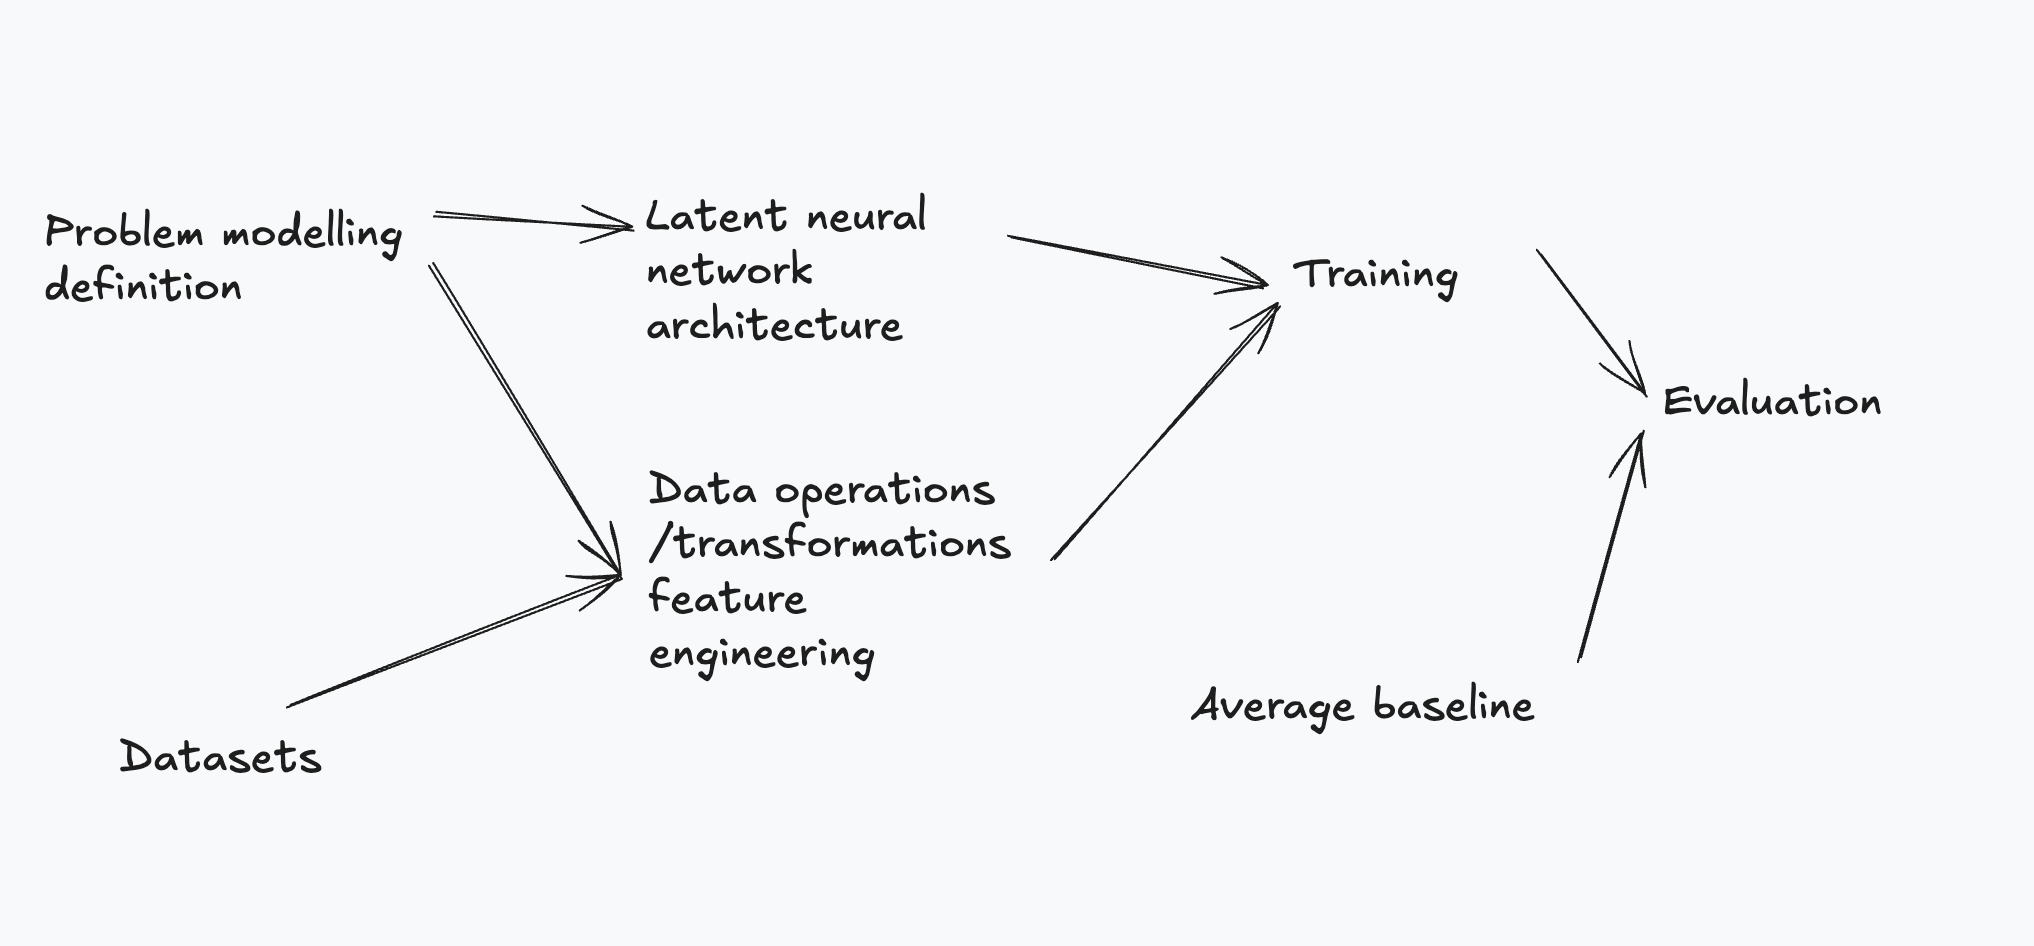
\includegraphics[width=1.5\textwidth]{diagram}
    \caption[Problem modelling overview]{Chapter content overview. }
\end{figure*}

The issue introduced in \ref{ch:problem}


\section{Methodology}

Given existing sessions data and data landscape from \autoref{ch:data}. Predicting power demand for various factors for any location in prague as mentioned in \autoref{ch:problem}. Utilizing existing data. So machine learning plus addition of some more insight.

So we are interested in predicting average profile for given charger given some temporal characteristic. Like month or day of the week.


\section{Latent Nerual Network Architecture}

\todo{mention relevant literature for the latent network from literatrue research}

\begin{figure}[hb]
    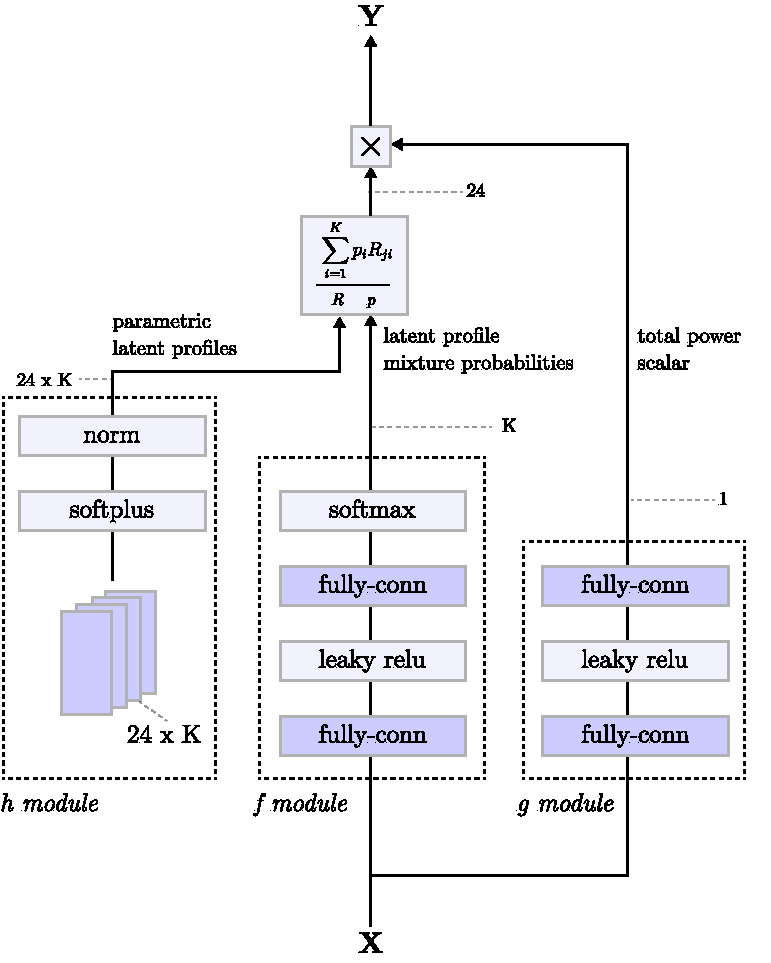
\includegraphics[width=0.7\textwidth]{nn-latent-architecture.pdf}
    \caption[Latent Neural Network Architecture]{Latent neural network architecture. Light blue rectangles denote NN layers without trainable parameters. While blue denotes layers with parameters learned by SGD. }
    \label{fig:nn-latent}
\end{figure}



\todo{mentions operations done to the data plus anaylsis of statistical impact of features on result}

\section{Input data transformation}

Standardization mainly.

\section{Training}

\todo{train test split, mention to be sure that we are learning on unseen data. So mby how there are multple chargers for one point}

\section{Baseline}

To be able to tell if our results have some value.
Are we better than average ? Because noone has done it for prague and even our greenfield problem formulation.